\chapter{Bose-Hubbard model} \label{app:bhModel}
When bosons are confined to the lowest energy band of a lattice, a particularly simple model known as the Bose-Hubbard Hamiltonian is used to describe the lattice system \cite{Jaksch1998}. 
	\begin{equation} \label{eq:boseHubbard}
		 H_{BH} = -J \sum_{\left< i,j \right>} \left(\hat{b}^{\dagger}_i \hat{b}_j + \hat{b}^{\dagger}_j \hat{b}_i \right)
		 		  + \frac{U}{2} \sum_i \hat{n}_i(\hat{n}_i - 1)
	\end{equation}
Where $\left< i,j \right>$ denotes a sum over nearest-neighbors. This model is the simplest example of a non-trivial interacting many-body system for dynamics in a lattice. The first term describes hopping of bosons from site to site at a rate $J/ \hbar$. The second term describes an interaction energy which is related to the s-wave contact interaction term, $g = 4 \pi \hbar^2 a_s/m$, where $a_s$, is the s-wave scattering length of the particles. $J$ and $U$ can be calculated directly using the Wannier functions of Eq.\;\ref{eq:wannier} and are given by \cite{Jaksch2005}
	\begin{equation} \label{eq:JandU}
	\begin{aligned}
		 J_{ij} &= - \int d^3x \; w_0(x-x_i) \left( \frac{p^2}{2m}+V(x) \right) w_0(x-x_j)\\
		 U &= \frac{4 \pi \hbar^2 a_s}{m} \int d^3x \; \left| w_0(x-x_i)\right|^4
	\end{aligned}
	\end{equation}
Using Eq.\;\ref{eq:JandU} we have calculated the expected tunneling rates and interaction energies for atomic strontium and plot the results in Fig.\;\ref{fig:fig_JandU} for homonuclear samples of strontium as a function of lattice depth. This single band calculation is valid under the assumption that the interaction energy of a site is smaller than the bandgap between the $n= 0$ and $1$ bands, namely $U N \lesssim \hbar \omega_{ho}$ where $N$ is the mean number of particles per site and $\hbar \omega_{ho}$ is the approximate energy spacing between bands \cite{Rey2004}. 


\begin{figure} \label{fig:fig_JandU}
	\centerline{
	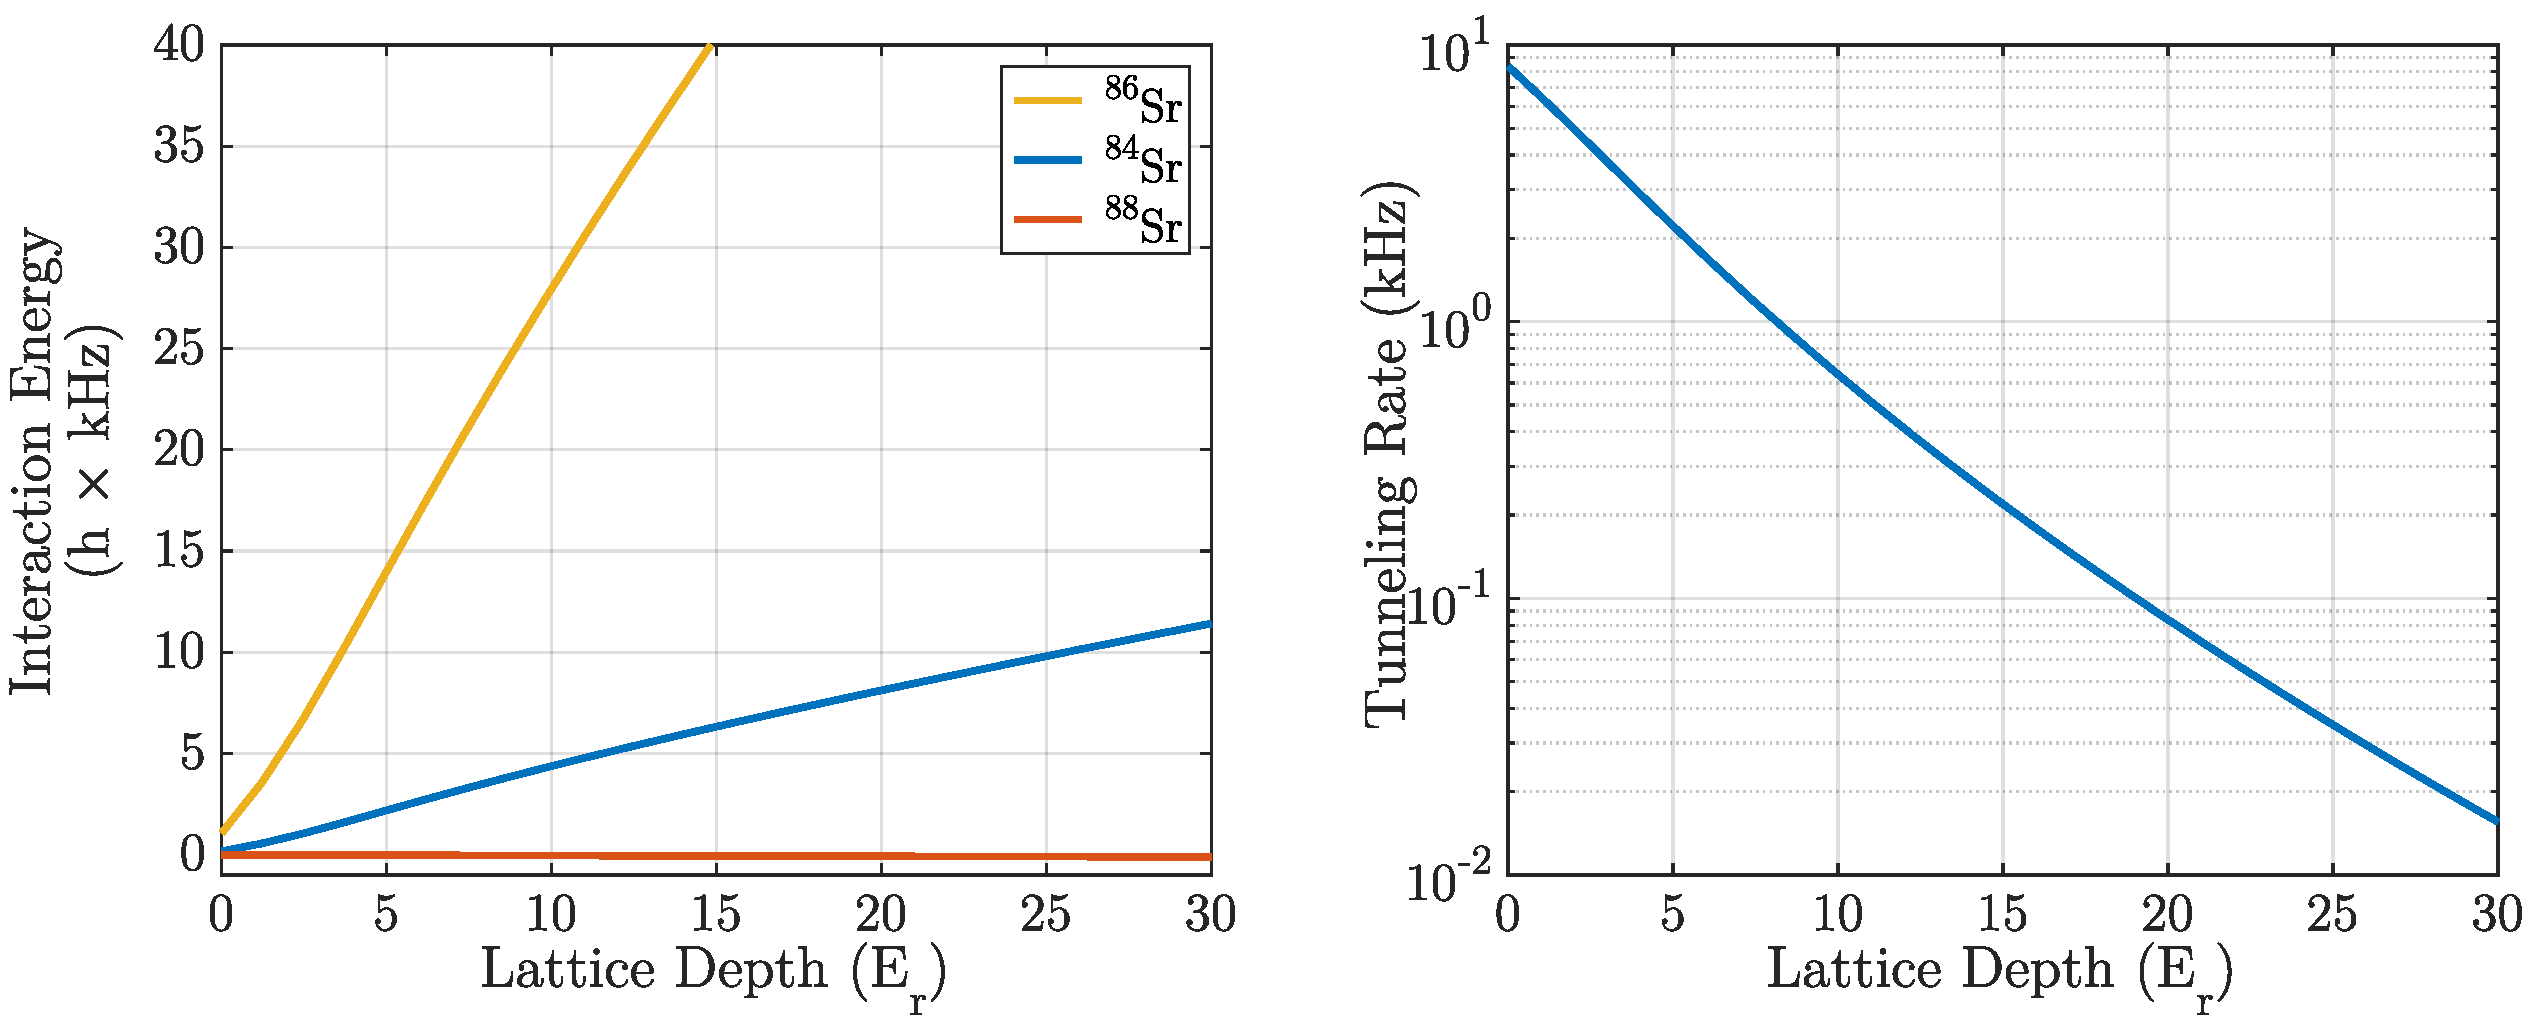
\includegraphics[width=\textwidth]{JandU.pdf}}
	\caption{Calculated interaction energies and tunneling rates for each isotope of strontium}{The interaction energy shows a large variation because of its dependence on the s-wave scattering length. However, the tunneling rate is approximately the same for all isotopes since the change in mass is negligible between isotopes.}
\end{figure}
	
	
Alternatively, Eq.\;\ref{eq:JandU} can be simplified through considering appropriate limits to the Bose-Hubbard model. In the limit that $U\!\rightarrow\!0$, the Bose-Hubbard model becomes exactly solvable and the energy of the $n=0$ band is given by $E_q^{(0)}=-2J \cos(q a)$ \cite{Jaksch2005}. Thus, the tunneling rate, $J$, can be related to the bandwidth of the lowest band as expressed in Eq.\;\ref{eq:JandU_simple}. Under a separate limit, $V_{lat}\,\rightarrow\,\infty$, then the tunneling rate goes to zero and the localized wavefunctions can be approximated by a Gaussian wavefunction which yields the form for the on-site interaction $U$ given in Eq.\;\ref{eq:JandU_simple} \cite{Rey2004}.
	\begin{equation} \label{eq:JandU_simple}
	\begin{aligned}
		 J &= \frac{E_{q=\hbar k_L} - E_{q=0}}{4}\\
		 U &= \frac{\hbar a_s}{\sqrt{2 \pi}}\frac{\bar{\omega}_{ho}}{\bar{a}_{ho}}
	\end{aligned}
	\end{equation}
Here $\bar{a}_{ho}$ and $\bar{\omega}_{ho}$ are the geometric means of the one-dimensional harmonic oscillator length and frequency given previously.

Competition between $J$ and $U$ results in a phase transition known as the superfluid - Mott insulator transition \cite{Fisher1989,Greiner2002}. When $J/U \gg 1$ atoms are free to delocalize over the lattice and the many-body ground state is a superfluid. In the opposite limit that $J/U \ll 1$, particle fluctuations between sites are no longer energetically accessible and the system transitions into an interaction induced insulating state known as a Mott insulator. This state is characterized by fixed particle number per site and in a 3D cubic lattice near unit filling, this phase transition occurs at $J/U \approx 35$ which, for $^{84}$Sr, corresponds to a lattice depth of $V_{lat} \approx 13E_r$ \cite{Fisher1989}.
